\documentclass[11pt]{article}

% ---------------------------------------------------------------- packages
\usepackage[letterpaper,margin=1in]{geometry}
\usepackage[T1]{fontenc}
\usepackage{lmodern}
\usepackage{microtype}
\usepackage{amsmath,amssymb}
\usepackage{graphicx}
\usepackage{booktabs}
\usepackage{tabularx}
\usepackage{multirow}
\usepackage{xcolor}
\usepackage{caption}
\usepackage{subcaption}
\usepackage[numbers,sort&compress]{natbib}
\usepackage[colorlinks=true,linkcolor=blue!50!black,citecolor=blue!50!black,urlcolor=blue!50!black]{hyperref}
\usepackage{enumitem}
\setlist{nosep,leftmargin=*}
\graphicspath{{../figures/}}
\captionsetup{font=small,labelfont=bf}

\newcommand{\Rthr}{$R_{\mathrm{thr}}$}
\newcommand{\pstar}{$p^{*}$}

\title{When Is Quantum Error Mitigation Worth Paying For?\\[2pt]
\large A Pre-Registered Study of Selective Mitigation for Noisy Variational Quantum Fraud Classifiers}

\author{Mayank Kumar Pokhriyal \and Tushar Poonia\\[4pt]
\small Katz School of Science and Health, Yeshiva University, New York, NY, USA\\
\small M.S.\ in Artificial Intelligence --- Capstone Research}

\date{Manuscript draft, October 2026 (not peer reviewed)}

\begin{document}
\maketitle

% ================================================================ abstract
\begin{abstract}
Quantum error mitigation trades additional circuits and shots for less biased estimates, but a deployed quantum classifier must decide \emph{when} that trade is worth making and \emph{which} technique to buy.
We study this decision for 4-qubit variational quantum classifiers (VQCs) that score credit-card transactions for fraud, under simulated depolarizing, thermal-relaxation and readout noise.
Each execution context can be served by no mitigation, tensored readout mitigation, zero-noise extrapolation (ZNE), both, or three times the shots; the cost-aware reference choice is the cheapest action whose Brier score is within 10\% of the best.
In a characterization of a single model, noise mainly damaged calibration and fixed-threshold decisions while leaving discrimination (AUPRC, AUROC) and the top-ranked frauds essentially intact, and mitigation repaired calibration without improving the area under the precision--recall curve beyond a shot-matched baseline.
We then tested, in three pre-registered stages, whether \emph{learning} the per-context decision from cheap label-free probes outperforms a simple rule.
Across 64 independently trained VQCs, pre-registered gates under near-categorical and under continuous joint noise found no \emph{material} residual decision structure beyond a simple probe rule, so no learned controller was trained.
On a sealed set of unseen model structures, opened once, a two-threshold probe rule fitted on training models made material errors in 2.0\% of decisions under continuous joint noise (95\% CI 1.5--2.6\%) and 8.8\% under categorical noise, matching the reference Brier score within 0.03\% at 0.6\% more shots.
Four pre-specified learned comparators did not reduce material errors, although the best of them disagreed less often with the reference choice; the intervals rest on only four held-out structures.
In the studied setting, selective mitigation reduces to a simple observable rule.
The evidence is simulation-only and we make no quantum-advantage claim.
\end{abstract}

% ================================================================ 1
\section{Introduction}

Near-term quantum processors are noisy \citep{preskill2018quantum}.
Quantum error mitigation (QEM) reduces the bias that noise introduces into estimated expectation values, at the price of additional quantum resources \citep{temme2017error,kandala2019error,cai2023quantum}.
Two widely used techniques are \emph{readout mitigation}, which inverts a calibrated model of measurement errors \citep{bravyi2021mitigating,maciejewski2020mitigation}, and \emph{zero-noise extrapolation} (ZNE), which amplifies gate noise---for example by pulse stretching \citep{kim2023scalable} or unitary folding \citep{giurgicatiron2020digital}---and extrapolates measured values to the zero-noise limit.
Neither is free: ZNE multiplies shots and two-qubit-gate exposure, and the benefit of mitigation depends on the platform and the budget \citep{russo2023testing,zhang2026worse}.

For a deployed quantum classifier this creates a recurring \emph{decision}: in the current execution context, should the system spend extra resources on mitigation, on which technique, or simply on more shots?
A natural proposal is to \emph{learn} this decision.
Recent work selects or tunes mitigation with contextual bandits and orchestration policies \citep{szachara2026gsc,rahman2026adaptive,majid2026context}.
These works report gains mainly over fixed (static) mitigation choices and, in one case, over grid-search and other published ZNE variants \citep{rahman2026adaptive}; to our knowledge none compares against a simple observable rule.
A decision-aware analysis suggests that accuracy gains from mitigation need not improve downstream decisions \citep{scavino2026decision}, and a budget-aware evaluation shows that mitigation can increase error relative to the raw estimate \citep{zhang2026worse}.
Whether learning is necessary therefore depends on how much structure the decision actually has once cheap observable signals are available---a question that, to our knowledge, has not been tested against simple rules on held-out models under pre-registration.

We study this question for variational quantum classifiers \citep{havlicek2019supervised,schuld2020circuit} that score credit-card transactions for fraud \citep{dalpozzolo2015calibrating,mlgulb2018creditcardfraud}.
Our research question is: \emph{When should a noisy quantum fraud classifier spend additional quantum resources on mitigation, and is learning that decision better than a simple observable rule?}

\paragraph{Contributions.}
\begin{enumerate}
\item A characterization showing that, for the studied 4-qubit VQCs, simulated noise primarily damages calibration and fixed-threshold decisions while leaving discrimination essentially intact, and that mitigation repairs calibration but does not improve the area under the precision--recall curve (AUPRC) beyond a shot-matched baseline (Section~\ref{sec:char}).
\item A leakage-safe counterfactual benchmark: 64 independently trained VQCs, every model run under every action (none, readout mitigation, ZNE, both, extra shots) with paired random draws, in near-categorical and continuous joint noise, with the policy context restricted to label-free probes and static descriptors (Sections~\ref{sec:formulation}--\ref{sec:methods}).
\item A three-stage pre-registered test of the learned-controller hypothesis---two gates and a one-time sealed held-out evaluation---showing that a two-threshold probe rule is near-Oracle on material errors and that pre-specified learned comparators did not reduce them (Sections~\ref{sec:policies}--\ref{sec:ablation}).
\end{enumerate}
All experiments were pre-registered and pushed to version control before their outcomes existed; negative results are reported as results.
We make no claim of quantum advantage: classical models score higher on the same inputs (Section~\ref{sec:arch}).

% ================================================================ 2
\section{Related Work and Research Gap}
\label{sec:related}

\paragraph{Quantum error mitigation.}
Zero-noise extrapolation was introduced with Richardson extrapolation \citep{temme2017error}, demonstrated on hardware \citep{kandala2019error}, and scaled to tens of qubits \citep{kim2023scalable}; digital ZNE realizes noise amplification by unitary folding \citep{giurgicatiron2020digital}.
Probabilistic error cancellation with learned sparse noise models removes bias at an exponential sampling cost \citep{vandenberg2023probabilistic}.
Readout mitigation by tensored or tomographic inversion \citep{bravyi2021mitigating,maciejewski2020mitigation} is inexpensive when calibration is amortized over a batch.
Cai et al.\ review the field \citep{cai2023quantum}.
A resource-normalized evaluation across hardware platforms finds mitigation beneficial on average but strongly platform-dependent, with some settings worse than no mitigation \citep{russo2023testing}; at a matched online shot budget, unconstrained ZNE can be worse than the raw estimate on a large fraction of instances \citep{zhang2026worse}.
In hybrid quantum neural networks, the benefit of system-level mitigation depends strongly on the noise model and its strength \citep{minguenjiki2026robustness}.
We therefore compare every mitigation action with a shot-matched alternative.

\paragraph{Learning for error mitigation.}
Learning-based QEM learns the \emph{mitigation map itself}, for example quasi-probability compensation from near-Clifford training circuits \citep{strikis2021learning} or regression models that emulate ZNE at lower cost \citep{liao2024machine}.
Relatedly, noise-aware circuit learning optimizes the circuit itself against a device's noise model \citep{cincio2021machine}.
Our question differs: we keep standard mitigation maps and ask only \emph{which one to apply, if any}.

\paragraph{Adaptive selection of mitigation.}
Several recent works select mitigation per context.
GSC-QEMit combines telemetry clustering, degradation forecasting and Thompson sampling to choose abstract mitigation intensities on eight simulated benchmark workloads, including GHZ, QFT and Grover \citep{szachara2026gsc}.
A cost-aware contextual bandit selects ZNE scale-factor sets for hybrid variational classifiers \citep{rahman2026adaptive}.
An orchestration policy selects among no mitigation, ZNE, probabilistic error cancellation, Clifford data regression and readout mitigation in quantum reinforcement learning for vehicle routing \citep{majid2026context}.
Rao et al.\ predict circuit fidelity from label-free circuit and hardware features and use a fuzzy-logic selector to choose between no mitigation, dynamical decoupling and ZNE \citep{rao2026adaptive}.
Scavino argues that mitigation should be selected by its effect on downstream decisions rather than by expectation-value accuracy, and finds that, in the regimes evaluated, decision-aware selection often retains the raw estimate \citep{scavino2026decision}.

\paragraph{Gap.}
To our knowledge, (i) none of these works places \emph{extra shots} and \emph{combined} mitigation in the same action space; (ii) the three learned selectors condition on information that is label-dependent or unavailable at deployment (ideal-state fidelity, simulator noise parameters, task loss, accuracy or reward), whereas the label-free selector of Rao et al.\ is hand-designed; and (iii) none compares a selector against a simple observable rule on held-out models under pre-registration.
We contribute that comparison; in our setting its answer does not favour learning.

\paragraph{Quantum machine learning for fraud detection.}
Variational, kernel and hybrid quantum classifiers have been applied to fraud detection on the same public dataset and on other transaction data \citep{elalami2026comparative,das2025qfdnn,tudisco2024evaluating,li2025hqrnn,kyriienko2022unsupervised}.
Comparisons with classical models are mixed: on the same dataset, tuned classical baselines outperform 4-qubit VQC and quantum-kernel classifiers \citep{dinut2026comparative}, whereas other studies report quantum or hybrid models matching or exceeding classical baselines on particular metrics or datasets \citep{kyriienko2022unsupervised,li2025hqrnn,tudisco2024evaluating}.
Noise can even improve some quantum models in specific regimes \citep{zhu2026rethinking,ahmed2025noisy}.
We use the VQC as a noisy classifier whose mitigation decisions we study, not as a competitor to classical fraud models.

% ================================================================ 3
\section{Problem Formulation}
\label{sec:formulation}

\paragraph{Contexts and actions.}
A \emph{context} $c$ is a triple (model $m$, noise environment $n$, shot budget $S$).
For each context the system chooses an action $a \in \{A0, A1, A2, A3, A4\}$:
A0 runs the circuit with $S$ shots; A1 adds tensored readout mitigation; A2 applies ZNE; A3 applies readout mitigation at every folding scale followed by ZNE; A4 runs the unmitigated circuit with $3S$ shots (the shot-matched alternative to ZNE).
Costs are accounted in shots, circuits, two-qubit-gate shots and calibration overhead (Table~\ref{tab:actions}); the induced cost order is $A0 < A1 < A4 < A2 < A3$.

\paragraph{Reliability endpoint.}
The model outputs fraud probabilities $p = (1-\langle O\rangle)/2$ for a Pauli-$Z$-type observable $O$.
Because noise acts mainly on calibration (Section~\ref{sec:char}), the primary endpoint is the Brier score \citep{brier1950verification} of the mitigated probabilities on the context's transaction panel, averaged over 20 finite-shot replicates.

\paragraph{Cost-aware Oracle.}
Let $B_c(a)$ be the context-mean Brier score of action $a$ and $B^{*}_c = \min_a B_c(a)$.
The Oracle action is the \emph{cheapest} action within a relative tolerance $\varepsilon$ of the best,
\begin{equation}
p^{*}(c) = \min_{\prec}\{a : B_c(a) \le (1+\varepsilon)\,B^{*}_c\}, \qquad \varepsilon = 0.10,
\end{equation}
where $\min_{\prec}$ follows the cost order.
Because \pstar\ is the cheapest action within tolerance, any other action is either outside the tolerance (if cheaper) or later in the registered cost order; a policy \emph{fails} at $c$ exactly when it disagrees with \pstar.
A failure is \emph{material} when the chosen action's Brier exceeds $(1+2\varepsilon)B^{*}_c$ or it costs at least $S$ more shots per inference than \pstar.
Near-ties and near-free overspends (e.g.\ A3 instead of A2, which adds only two calibration circuits per batch) are therefore failures but not material ones.
We also report relative Brier regret $(B_c(a)-B_c(p^{*}))/B^{*}_c$ and cost regret in units of $S$.
Brier regret can be negative: \pstar\ may lie up to $\varepsilon$ above the best Brier score, so a policy that overspends (for example always-A3) can be more reliable than the Oracle while costing more.
Cost regret and the overspend criterion count action shots only; reported shots per inference also include probe shots.

\paragraph{Observable context.}
A policy sees only (i) 16 static model descriptors (circuit size and depth, ansatz, readout observable, encoding family, feature set, frozen clean-validation metrics and threshold) and (ii) 11 features from two label-free probes executed each batch: a \emph{readout probe}---the two calibration circuits that A1/A3 reuse---and a \emph{gate probe}---32 fixed synthetic parameter bindings executed at folding factors 1 and 3, summarized by mean $|\langle O\rangle|$, its contraction and slope.
The probes cost $66S$ shots per batch, charged to every probing policy.
True noise parameters, noise labels, design-point and model identifiers, labels and post-action outcomes are offline-only; a feature registry and automated tests prevent them from entering any policy input table.
The probes are deployable measurements that \emph{estimate} the noise, by design: the readout probe tracks the true mean readout error closely.

% ================================================================ 4
\section{QML Fraud-Detection Architecture}
\label{sec:arch}

\paragraph{Data and leakage-safe partitions.}
We use the public European credit-card fraud dataset \citep{dalpozzolo2015calibrating,mlgulb2018creditcardfraud} (284{,}807 transactions, 0.17\% fraud).
After removing exact duplicates, 283{,}726 rows and 473 frauds remain.
Rows that are identical apart from the timestamp are kept together, and a group-aware stratified split assigns five disjoint partitions (Table~\ref{tab:partitions}).
All preprocessing is fitted on the VQC-training partition only; controller partitions are never used to fit a classifier.

\begin{table}[t]
\centering
\caption{Group-aware partitions after deduplication. Controller partitions serve the mitigation-policy study; the controller-test partition was sealed until the final evaluation.}
\label{tab:partitions}
\small
\begin{tabular}{lrrl}
\toprule
Partition & Rows & Frauds & Used for \\
\midrule
VQC train & 127{,}677 & 213 & fitting every VQC and preprocessing \\
VQC validation & 28{,}372 & 47 & model qualification, thresholds, characterization \\
Controller train & 42{,}559 & 71 & policy fitting (training models) \\
Controller validation & 28{,}372 & 47 & policy validation (validation models) \\
Controller test & 56{,}746 & 95 & sealed; opened once (test models) \\
\bottomrule
\end{tabular}
\end{table}

\paragraph{Variational quantum classifiers.}
Each classifier uses four input features angle-encoded into four qubits, a ZZ feature map \citep{havlicek2019supervised}, a RealAmplitudes or EfficientSU2 ansatz, and a parity or mean-$Z$ readout, trained by COBYLA on balanced subsets of the VQC-training partition.
A first model with a clipped $[-\pi,\pi]$ encoding learned weak signal (validation AUPRC 0.104); training-data diagnostics traced this to saturation and phase aliasing, and a pre-registered cross-validated repair selected a wide-range encoding with ansatz depth 2 (validation AUPRC 0.507, AUROC 0.957, Brier 0.0093).
Classical models on the same four inputs reach AUPRC 0.59--0.62 (point estimates; only the logistic-regression gap, $+0.113$ $[0.021, 0.214]$, has an interval excluding zero), so the VQC is a working but not advantageous classifier.

\paragraph{Model pool.}
To make models the independent unit of analysis, we trained a pre-registered pool of 64 VQCs: 16 structures (three feature sets, three alias-safe encodings, two ansatz families at two depths, parity and mean-$Z$ readouts) $\times$ 4 seeds.
All 64 qualified on clean validation data (median AUPRC 0.235, range 0.047--0.538; AUROC 0.91--0.96).
Predictions differ substantially between structures (median pairwise Spearman correlation 0.24) and little between seeds of one structure (0.91).
Structures were split 8/4/4 into training, validation and test models, keeping all seeds of a structure together; each model is evaluated on its own controller partition.
Each model's decision threshold was tuned once on clean validation data and frozen.

\begin{figure}[t]
\centering
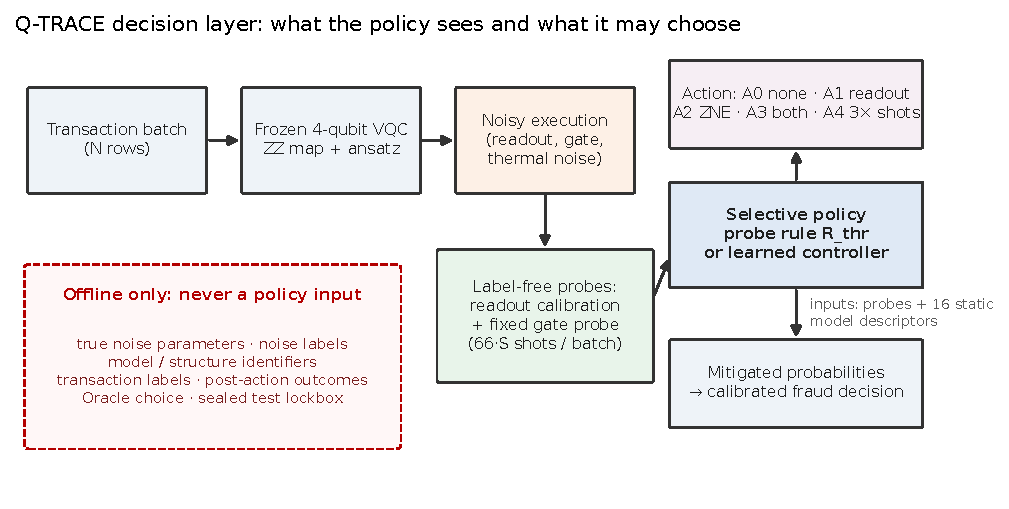
\includegraphics[width=\linewidth]{fig1_architecture.pdf}
\caption{The selective-mitigation decision layer. The policy observes only label-free probes and static model descriptors; all quantities in the dashed box are offline-only. Schematic; no data.}
\label{fig:architecture}
\end{figure}

% ================================================================ 5
\section{Noise Models and Experimental Methodology}
\label{sec:methods}

\paragraph{Noise simulation.}
Circuits are transpiled to $\{r_z, \sqrt{X}, X, \mathrm{CX}\}$ and simulated exactly with Qiskit Aer density matrices \citep{javadiabhari2024quantum}: depolarizing channels after one- and two-qubit gates (parameters $p_1, p_2$), thermal relaxation over gate durations of 35\,ns and 300\,ns ($T_1, T_2$), and per-qubit readout confusion ($p_{01}, p_{10}$) applied to the exact output distribution.
Finite-shot outcomes are multinomial draws from these distributions, paired across actions within a replicate.
Severities follow a low/medium/high anchor grid with $p_2$ up to 0.02, $T_1$ down to 50\,$\mu$s and mean readout error up to 0.05.
Asymmetric readout ($p_{10} > p_{01}$) is a \emph{synthetic} stress-test assumption, not device calibration data.

\paragraph{Two noise environments.}
\emph{Phase 5B} used eight near-categorical noise conditions: clean, three readout-only, two gate-only and two combined.
\emph{Phase 5C} varied all sources continuously and jointly: each source was placed on an anchor-severity scale $s\in[0,3]$, piecewise linear through the none, low, medium and high anchors so that no point exceeds the validated ``high'' anchor, and a split-plot space-filling design crossed 17 gate settings (a gate-free setting and a 16-point maximin Latin hypercube in depolarizing $\times$ thermal severity) with four readout settings each (a sliced Latin hypercube in magnitude $\times$ asymmetry), giving 68 noise points.
Phase 5B used budgets of 1{,}024 and 4{,}096 shots; Phase 5C added 256 shots.
Both used 20 replicates per context.

\paragraph{Scale.}
Phase 5B produced 102{,}400 counterfactual action outcomes (122{,}880 rows including a shot-matched diagnostic for ZNE) and Phase 5C 1{,}305{,}600; the controller-test rows of both were written to a sealed, version-control-ignored store and only their row counts and content hashes were committed.

\paragraph{Pre-registration and gates.}
Every phase was pre-registered with its configuration and code, pushed before any outcome existed, and executed as a ``reported'' run on a clean source tree.
Gates decided whether to proceed (Figure~\ref{fig:workflow}).
In particular, a learned controller was to be trained only if a \emph{residual-complexity gate} found decision structure that the best pre-registered simple rule could not capture.

\begin{figure}[t]
\centering
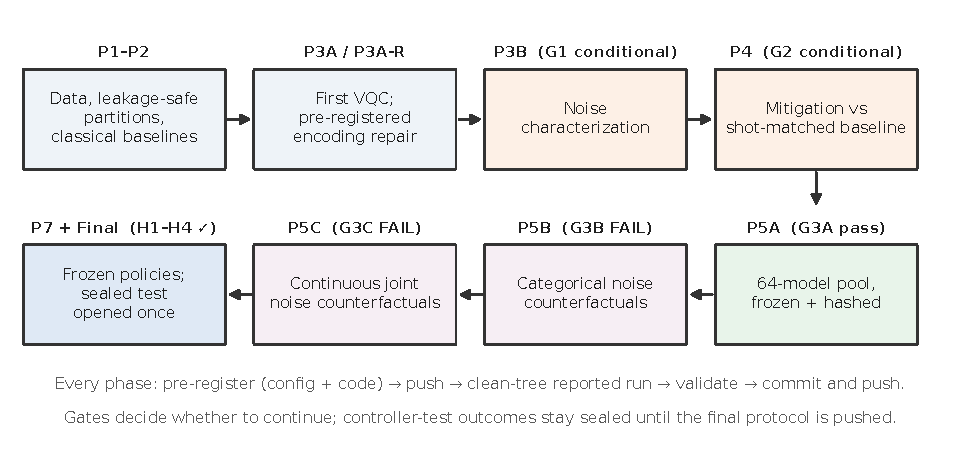
\includegraphics[width=\linewidth]{fig2_workflow.pdf}
\caption{Pre-registered workflow. Each gate's outcome is shown in parentheses; the sealed controller test was opened once after the final protocol had been pushed. Schematic; no data.}
\label{fig:workflow}
\end{figure}

% ================================================================ 6
\section{Error-Mitigation Strategies}
\label{sec:mitigation}

\paragraph{Readout mitigation (A1).}
Two calibration circuits ($|0000\rangle$ and $|1111\rangle$) estimate per-qubit confusion matrices from counts only; the tensored inverse is applied to measured frequencies and rows with negative quasi-probabilities are projected onto the probability simplex in Euclidean norm.
The calibration is amortized over the batch.

\paragraph{Zero-noise extrapolation (A2).}
The transpiled circuit $U$ is globally folded to $U(U^{\dagger}U)^{k}$ at noise scales $\lambda\in\{1,3,5\}$ \citep{giurgicatiron2020digital}; the expectation value is extrapolated to $\lambda=0$ with a linear least-squares fit (weights $13/12, 1/3, -5/12$) and clipped to the physical range.

\paragraph{Combined (A3) and extra shots (A4).}
A3 applies readout mitigation at every scale before extrapolation.
A4 spends the same $3S$ shots as ZNE on the unfolded circuit, isolating the value of variance reduction from bias removal.

\begin{table}[t]
\centering
\caption{Actions and resources per logical inference ($S$ shots per circuit, $N$ transactions per batch). CX exposure is relative to A0.}
\label{tab:actions}
\small
\begin{tabular}{llccc}
\toprule
Action & Description & Shots & Circuits & CX exposure \\
\midrule
A0 & none & $S$ & 1 & $1\times$ \\
A1 & tensored readout mitigation & $S + 2S/N$ & $1 + 2/N$ & $1\times$ \\
A4 & extra shots (unmitigated) & $3S$ & 1 & $3\times$ \\
A2 & ZNE, global folding $\lambda\in\{1,3,5\}$ & $3S$ & 3 & $9\times$ \\
A3 & readout mitigation + ZNE & $3S + 2S/N$ & $3 + 2/N$ & $9\times$ \\
\bottomrule
\end{tabular}
\end{table}

\subsection{What noise and mitigation do}
\label{sec:char}

On the repaired base model (validation partition, exact simulation), noise at the anchor severities left discrimination essentially unchanged: the AUPRC changed by at most 0.003 for depolarizing, thermal and combined noise, with every 95\% interval containing zero, and at least 46 of the 47 top-ranked validation frauds were preserved.
Noise did reorder scores within the legitimate bulk (Kendall $\tau$ 0.96--0.99) and damaged calibration \citep{guo2017calibration}: the Brier score rose from 0.0093 to 0.121 under combined-high noise (Figure~\ref{fig:noise}).
Scores contracted toward 0.5; at the frozen threshold, precision fell from 0.53 to 0.03.
Symmetric readout noise is an exact affine contraction of $Z$-type scores and left ranking metrics unchanged to $10^{-16}$, a negative control that passed.

With 1{,}024 shots and 20 replicates (Figure~\ref{fig:mitigation}), no action improved AUPRC over its resource-matched comparator in any condition, whereas mitigation restored calibration: readout mitigation reduced the Brier score from 0.053 to 0.011 under high symmetric readout noise, ZNE from 0.055 to 0.038 under high depolarizing noise, and the combination from 0.122 to 0.054 under combined-high noise; three times the shots left the Brier score unchanged.
Linear ZNE recovered 13--70\% of the exact Brier gap to the clean model, and the fixed-threshold F1 score recovered by up to $+0.30$ (1{,}024 shots) and $+0.34$ (4{,}096 shots).
The cost-aware best action depended on the noise family---none for clean, readout mitigation for readout noise, ZNE for gate noise and both for combined noise---and was identical at both budgets.

\begin{figure}[t]
\centering
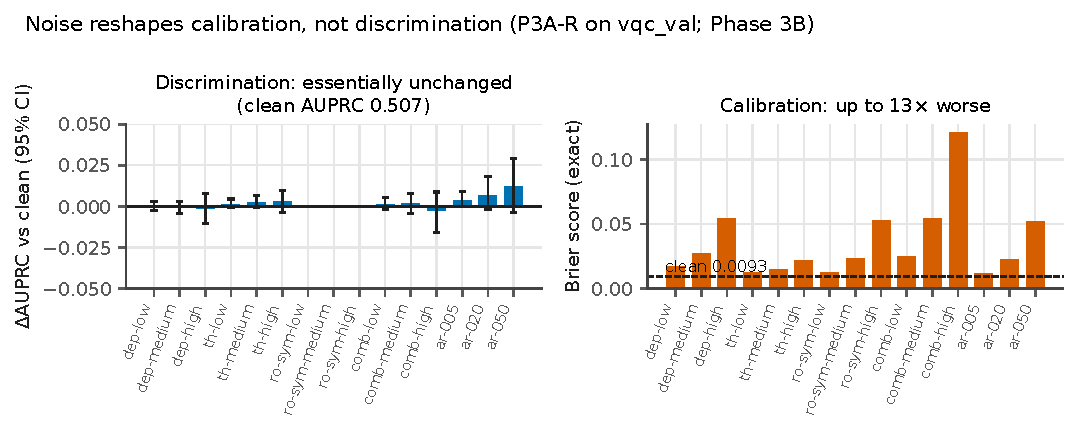
\includegraphics[width=\linewidth]{fig3_noise_effects.pdf}
\caption{Noise changes calibration, not discrimination (repaired base model, validation partition, exact simulation). Left: change in AUPRC with 95\% paired bootstrap intervals. Right: Brier score; the dashed line is the clean model.}
\label{fig:noise}
\end{figure}

\begin{figure}[t]
\centering
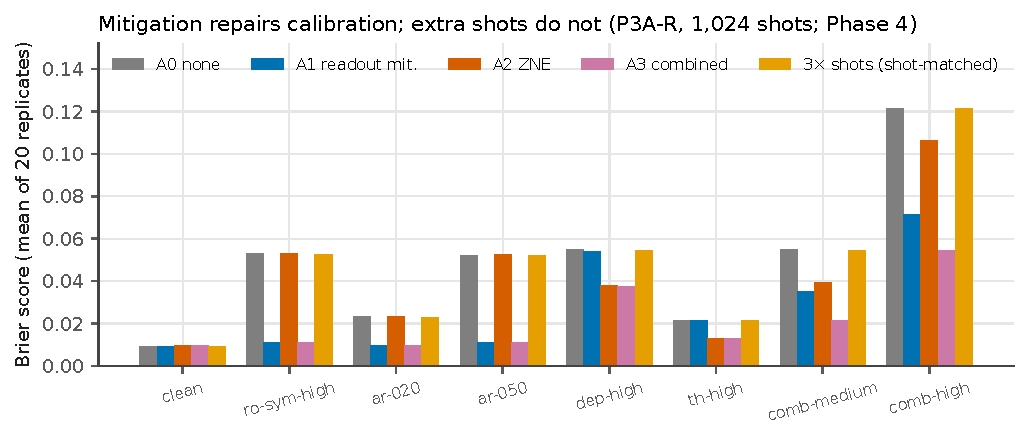
\includegraphics[width=\linewidth]{fig4_mitigation.pdf}
\caption{Brier score by condition and action (1{,}024 shots, mean of 20 replicates). Mitigation removes calibration bias; three times the shots do not.}
\label{fig:mitigation}
\end{figure}

% ================================================================ 7
\section{Learned-Controller and Deterministic-Policy Comparisons}
\label{sec:policies}

\paragraph{Deterministic policies.}
Universal policies always choose one action.
Three simple probe rules share a four-cell decision list: readout noise is detected when the readout-probe error is at least $t_r$, gate noise when the gate-probe contraction is at most $t_g$, and each cell (none, gate, readout, both) takes the majority Oracle action among training replicates.
$R_{\mathrm{cat}}$ uses a-priori thresholds ($t_r=0.005$, $t_g=0.90$); \Rthr\ chooses $(t_r,t_g)$ per shot budget by minimizing training failure over a $39\times39$ quantile grid; $R_{\mathrm{obs}}$ fits \Rthr\ separately for parity and mean-$Z$ readouts.
All rules are fitted on training models only.

\paragraph{Learned comparators.}
Four learned comparators, specified before fitting, use all 27 registered inputs: multinomial logistic regression, a depth-3 decision tree, and histogram gradient boosting (depth 4, learning rate 0.1, 200 iterations), each predicting \pstar\ directly, plus the same gradient boosting predicting each action's log Brier ratio to A0 followed by the cost-aware rule.
Hyperparameters are fixed in advance; the comparators are fitted on training models only and frozen by committed fingerprints of their decisions.

\paragraph{Gates.}
\emph{G3B} (Phase 5B) failed if the category rule's validation failure was below 5\%.
\emph{G3C} (Phase 5C) passed to controller training only if (1) at least two actions were each preferred in $\ge10\%$ of contexts, (2) the best simple rule failed in $\ge15\%$ of validation decisions, (3) the residual depended on the model at a fixed noise point across several structures, (4) it exceeded replicate label noise by $\ge0.10$, (5) material failures were $\ge10\%$, and (6) support was adequate; it failed if the best rule's material failure was below 5\%.

\paragraph{Phase 5B result.}
Under near-categorical noise the Oracle action was a lookup on the noise family.
A four-cell category rule fitted on training structures failed in 0.33\% of validation replicates, against 62.5\% for the best single action.
Mitigation benefit was strongly model-specific in magnitude (intraclass correlation about 0.98 for the readout-based actions), but the noise context explained 82--99\% of its variance and rarely changed which action won.
Three times the shots was never preferred.
The residual association between structure and preferred action was statistically detectable (mutual information 0.08~nats, $p=0.001$) but far below materiality.
G3B failed, so no controller was trained.

% ================================================================ 8
\section{Continuous Mixed-Noise Experiments}
\label{sec:continuous}

Because Phase 5B's conditions were near-categorical, its probes effectively read the category.
Phase 5C asked whether continuous joint noise creates a harder decision.
It instead removed most of the choice (Figure~\ref{fig:preferred}).
In our design, 16 of the 17 gate settings carry gate noise; across all contexts, combined mitigation was the Oracle action in 67--71\% and ZNE alone in 23--27\% (71--76\% and 24--29\% of the contexts with gate noise); ZNE won where readout error was below about 0.003, and readout mitigation or no mitigation won only on the gate-free setting.
Three times the shots was never preferred at the registered tolerance (at most 0.03\% of contexts at $\varepsilon=0.20$), and changing the shot budget changed \pstar\ in under 3\% of model--point pairs.
Oracle labels were stable: split-half agreement was 0.98 and the bootstrap probability that a label changes was 0.9\%.

The best simple rule, \Rthr, disagreed with the Oracle in 9.6\% of validation replicates [8.0, 11.7], but only 2.0\% [1.6, 2.7] of its decisions were material, with relative Brier regret $+0.3\%$ $[-0.4, +1.0]$ and $0.02S$ of action-shot cost regret.
Even an optimistic model-agnostic policy that knew the \emph{true} noise point disagreed with the Oracle in only 5.8\% of validation contexts; the largest model dependence came from a mean-$Z$ training structure.
The residual association between structure and preferred action was again statistically detectable (validation mutual information 0.04~nats, $p<0.001$), driven by the mean-$Z$ readout, but small.
G3C failed on its pre-registered \emph{negligible-regret} condition, so no learned controller was trained.

\begin{figure}[t]
\centering
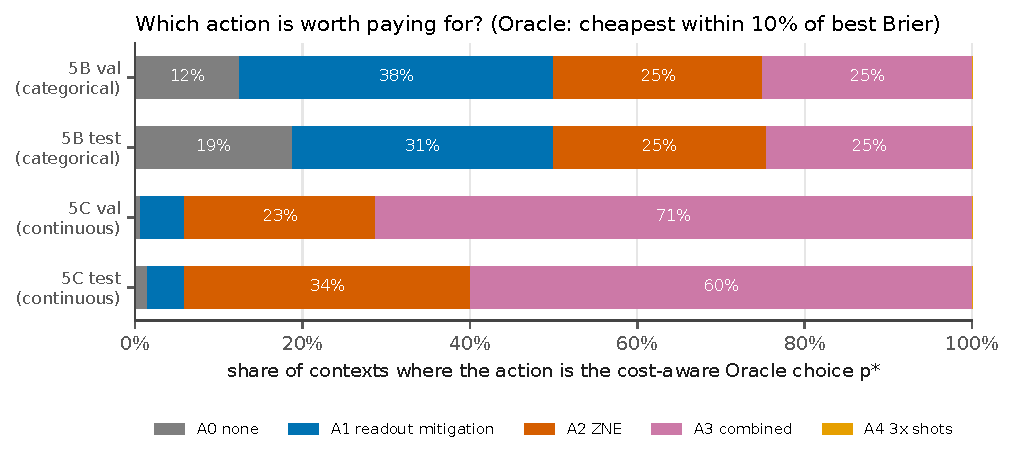
\includegraphics[width=\linewidth]{fig5_preferred_actions.pdf}
\caption{Share of contexts in which each action is the cost-aware Oracle choice. Under the continuous joint-noise design the decision collapses onto ZNE and combined mitigation; three times the shots is never preferred.}
\label{fig:preferred}
\end{figure}

% ================================================================ 9
\section{Statistical Evaluation and Resource Accounting}
\label{sec:stats}

\paragraph{Units and uncertainty.}
Models, nested in structures, are the independent units.
In the multi-model phases (5B onward), uncertainty is quantified by a two-stage cluster bootstrap (resampling structures, then models within each structure; 2{,}000 resamples); replicates, transactions and action rows are never treated as independent observations.
(The single-model characterization resamples transactions and replicates for one model and makes no claim beyond that model.)
Policy comparisons use paired, per-decision differences against \Rthr; we report them as comparator minus \Rthr, so positive values favour the rule.
The held-out test contains only four structures, so a percentile bootstrap at the structure level has few distinct resamples and its intervals are likely too narrow; the interval for always-A3 is degenerate.
The pre-registered detectable effect of about 0.70 standard deviations assumed 16 independent models; at the structure level, power is lower.

\paragraph{Resources.}
Costs are accounted per logical inference without collapsing them into one number: task shots, mitigation shots, calibration shots, circuits and two-qubit-gate shots.
Probing policies are charged the probe cost of $66S$ shots per batch; universal policies are not.
The probe cost includes the two readout-calibration circuits that A1/A3 also pay for, so probing policies are charged slightly conservatively.

\paragraph{Pre-specified hypotheses.}
On the sealed test: \textbf{H1} \Rthr's material failure $\le 0.05$ and relative Brier regret $\le 0.02$; \textbf{H2} (non-superiority) no learned comparator is meaningfully better, meaning neither lower material failure by $\ge0.02$ with a paired interval excluding zero nor $\ge5\%$ fewer shots at no more than $0.005$ additional material failure; \textbf{H3} \Rthr\ has lower material failure than every universal policy and uses no more shots than always-A3; \textbf{H4} (categorical environment) \Rthr's material failure $\le 0.10$.

% ================================================================ 10
\section{Held-Out Experimental Results}
\label{sec:results}

The sealed controller test---16 models from four structures never used for fitting or selection, including a mean-$Z$ structure---was opened once, after the protocol, the code and the frozen comparators had been pushed.
The stored outcomes matched their committed content hashes and the refitted learned comparators reproduced their frozen decision fingerprints.

All four hypotheses were supported (Table~\ref{tab:final}, Figures~\ref{fig:final} and~\ref{fig:cost}).
Under continuous joint noise, \Rthr\ made material errors in 2.0\% of decisions [1.5, 2.6] with relative Brier regret $-0.03\%$ (95\% CI $-1.7\%$ to $+1.2\%$), spending 0.6\% more shots than the Oracle and 3.4\% fewer than always using combined mitigation.
The best learned comparator on this test, gradient boosting, tied it (2.1\%); the paired difference in material failure (comparator minus \Rthr) was $+0.0005$ ($-0.016$ to $+0.027$), so the interval excludes a comparator advantage as large as the pre-registered 0.02 margin.
Under categorical noise, \Rthr's material failure was 8.8\%, inside the pre-registered bound; the category rule fitted on Phase 5B data did significantly better (6.4\%; paired difference $-0.024$, 95\% CI $-0.037$ to $-0.011$), and the learned comparators were worse (11.8--43.9\%, best: the depth-3 tree).

The learned comparators did have an advantage on the stricter, non-registered endpoint of \emph{any} disagreement with the Oracle.
On the continuous test, gradient boosting disagreed with the Oracle in 6.5\% of decisions against 21.9\% for \Rthr\ (paired difference $-0.154$ $[-0.391, -0.028]$), and the depth-3 tree and $R_{\mathrm{obs}}$ were also significantly closer to the Oracle.
These extra disagreements of \Rthr\ were not material.
The learned comparators were also unstable between validation and test: gradient boosting's material failure was 10.7\% on validation and 2.1\% on test, and the depth-3 tree's 17.5\% and 2.6\%, whereas \Rthr's was 2.0\% on both.

\Rthr's raw disagreement on the continuous test (21.9\%) was higher than on validation (9.6\%) while its material failure was unchanged.
The excess came from the unseen mean-$Z$ structure, where \Rthr\ adds readout mitigation that mean-$Z$ readouts barely need; the overspend is two calibration circuits per batch and was not material (1.4\%).
$R_{\mathrm{obs}}$, which conditions on the readout observable, absorbed it, whereas learned comparators trained on a single mean-$Z$ structure reached 5--30\% material failure on the new one (Figure~\ref{fig:learned}).

Always-A3's material failure, 5.9\%, equals exactly the share of contexts on the gate-free design setting (1/17), where it pays $2S$ more than readout mitigation.
H3's margin over always-A3 and \Rthr's 3.4\% shot saving therefore scale with the share of gate-free batches; on a device where gate noise is always present, both shrink towards the A2-versus-A3 choice, which costs two calibration circuits per batch.

\begin{table}[t]
\centering
\caption{One-time held-out evaluation (all shot budgets pooled). Material failure with 95\% two-stage cluster bootstrap intervals over four held-out structures (likely too narrow; see Section~\ref{sec:stats}); relative Brier regret against the Oracle (negative values mean more reliable than the cost-aware Oracle, at higher cost); total shots per inference including probes, relative to the Oracle.}
\label{tab:final}
\footnotesize
\setlength{\tabcolsep}{4pt}
\begin{tabular}{@{}lccccc@{}}
\toprule
& \multicolumn{4}{c}{Continuous joint noise (5C test)} & 5B test \\
\cmidrule(lr){2-5}\cmidrule(l){6-6}
Policy & \shortstack{Material\\failure} & \shortstack{Any dis-\\agreement} & \shortstack{Brier\\regret} & \shortstack{Shots vs.\\Oracle} & \shortstack{Material\\failure} \\
\midrule
Never mitigate (A0) & 0.960 & 0.986 & $+93.1\%$ & $0.35\times$ & 0.813 \\
Always A3 & 0.059 & 0.400 & $-1.4\%$ & $1.04\times$ & 0.500 \\
5B category rule $R_{\mathrm{cat}}$ & 0.045 & 0.249 & $+1.0\%$ & $0.99\times$ & 0.064 \\
\textbf{Probe rule \Rthr} & \textbf{0.020 [0.015, 0.026]} & \textbf{0.219} & $\mathbf{-0.03\%}$ & $\mathbf{1.006\times}$ & \textbf{0.088} \\
$R_{\mathrm{obs}}$ (+ readout type) & 0.021 [0.017, 0.025] & 0.089 & $+0.7\%$ & $1.006\times$ & 0.119 \\
Logistic (learned) & 0.094 & 0.173 & $+2.4\%$ & $0.95\times$ & 0.177 \\
Tree, depth 3 (learned) & 0.026 & 0.086 & $+0.7\%$ & $1.008\times$ & 0.118 \\
Gradient boosting (learned) & 0.021 [0.005, 0.044] & 0.065 & $+0.3\%$ & $1.009\times$ & 0.363 \\
GBT benefit model (learned) & 0.026 & 0.150 & $-0.26\%$ & $1.013\times$ & 0.439 \\
Oracle & 0 & 0 & 0 & $1\times$ & 0 \\
\bottomrule
\end{tabular}
\end{table}

\begin{figure}[t]
\centering
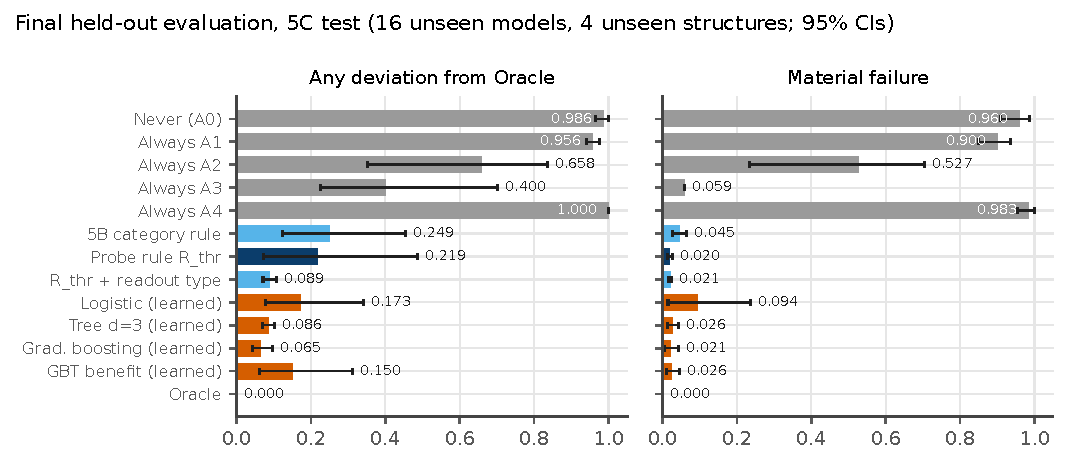
\includegraphics[width=\linewidth]{fig8_final_heldout.pdf}
\caption{One-time held-out evaluation under continuous joint noise (16 unseen models, four unseen structures). Bars: any disagreement with the Oracle (left) and material failure (right), with 95\% two-stage cluster intervals.}
\label{fig:final}
\end{figure}

\begin{figure}[t]
\centering
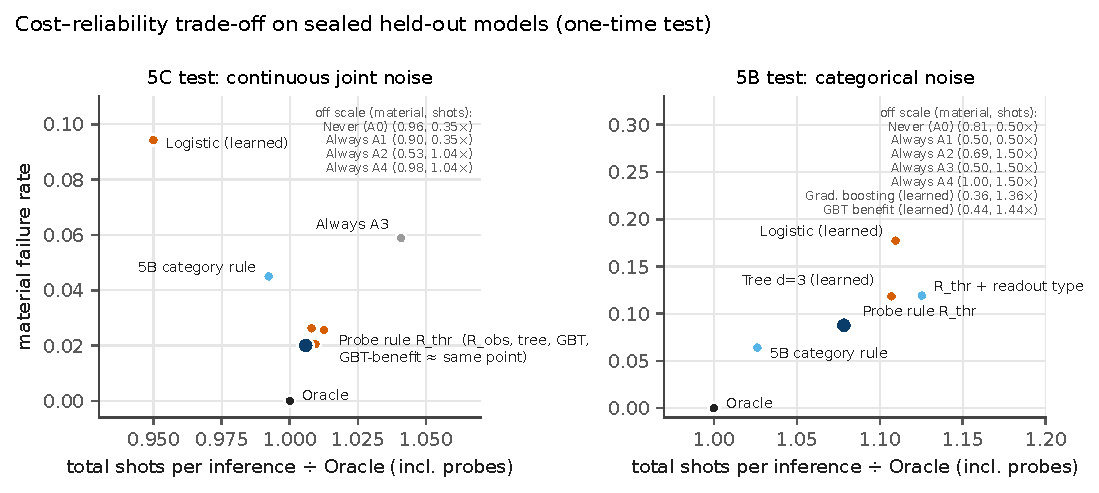
\includegraphics[width=\linewidth]{fig6_cost_reliability.pdf}
\caption{Cost--reliability trade-off on the sealed test. Policies far from the competitive region are listed in each panel with their (material failure, relative shots). Always-A3's material failure equals the gate-free share of the design.}
\label{fig:cost}
\end{figure}

\begin{figure}[t]
\centering
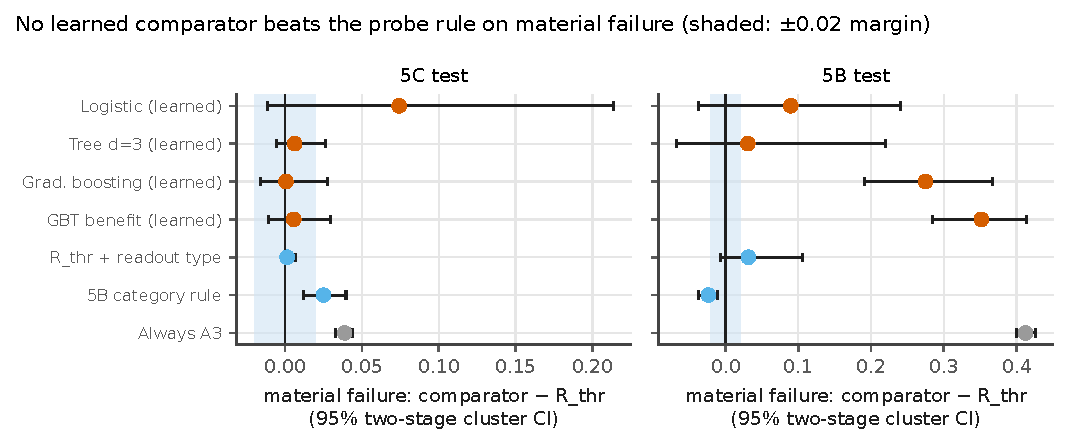
\includegraphics[width=\linewidth]{fig7_learned_vs_rule.pdf}
\caption{Paired difference in material failure, comparator minus \Rthr, with 95\% two-stage cluster intervals; positive values favour the rule. The shaded band is the pre-registered $\pm0.02$ margin. On the categorical (5B) test the 5B category rule $R_{\mathrm{cat}}$ is better than \Rthr.}
\label{fig:learned}
\end{figure}

% ================================================================ 11
\section{Ablation Studies}
\label{sec:ablation}

Ablations were run on validation data only; the sealed test was not reused.
Refitting \Rthr\ with only the gate probe left its material failure essentially unchanged (1.8\% under continuous noise, 9.4\% under categorical noise, although its raw disagreement with the Oracle rose from 10\% to 25\% under continuous noise), whereas a readout-only rule (6.2\%, 50\%) and a probe-free fixed action per budget (5.9\%, 50\%) were much worse (Figure~\ref{fig:ablation}).
The gate probe therefore carries the material decision---whether to pay three times the shots for ZNE-based mitigation---while the readout probe only chooses between ZNE and combined mitigation, which differ by two calibration circuits.
Because the probes cost $66S$ shots per batch, probing paid for itself relative to always using combined mitigation only for batches larger than about 645--685 transactions under continuous noise, depending on the budget (about 80 under categorical noise); our panels contained 28{,}372--56{,}746 transactions.
This break-even is conservative (the $66S$ include two calibration circuits that always-A3 already pays) and, like H3, it depends on the share of gate-free batches in the design.
Registered sensitivity analyses showed that the rule's material failure stayed between 2.0\% and 7.5\% for tolerances $\varepsilon$ between 0.05 and 0.20.

\begin{figure}[t]
\centering
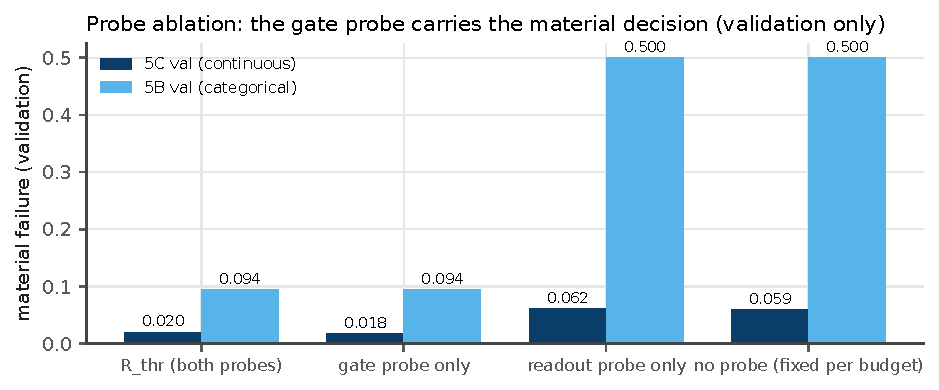
\includegraphics[width=\linewidth]{fig9_probe_ablation.pdf}
\caption{Probe ablation on validation data: on material failure, the gate probe alone recovers the full rule.}
\label{fig:ablation}
\end{figure}

% ================================================================ 12
\section{Limitations and Threats to Validity}
\label{sec:limitations}

\begin{itemize}
\item \textbf{Simulation only.} All noise is simulated; asymmetric readout is a synthetic assumption, and no crosstalk, drift, leakage or coherent errors are modelled. Hardware validation is the main external-validity gap.
\item \textbf{Scale.} Four qubits, shallow circuits (15--18 CX gates) and one public dataset with 0.17\% prevalence and features that are an inherited PCA.
\item \textbf{Models.} The VQCs are weaker than classical models on the same inputs; no quantum advantage is claimed or implied.
\item \textbf{Mitigation scope.} Only readout inversion and linear ZNE were studied; probabilistic error cancellation, Clifford data regression and dynamical decoupling may produce richer decisions.
\item \textbf{Probes and design.} The gate probe is insensitive to thermal relaxation (Spearman $-0.12$ with thermal severity); the rule relied on gate-noise presence, which depolarizing noise provided in 16 of 17 gate settings of our design. The advantage over always-A3 and the probing break-even scale with the share of gate-free batches.
\item \textbf{Thresholds and endpoints.} Per-model decision thresholds were tuned on clean validation data and are optimistic; the Oracle tolerance and the material-failure definition are design choices, fixed in advance and probed by sensitivity analysis.
\item \textbf{Power and intervals.} The held-out test spans four structures (one mean-$Z$); cluster-bootstrap intervals over four clusters are likely too narrow, and structure-level power is low. We do not claim universal generalization.
\item \textbf{Endpoint choice.} The registered endpoint is material failure. On raw disagreement with the Oracle, two learned comparators and $R_{\mathrm{obs}}$ were significantly closer to the Oracle than \Rthr; a different endpoint could favour them.
\end{itemize}

% ================================================================ 13
\section{Discussion and Future Research}
\label{sec:discussion}

\paragraph{Observed versus interpreted.}
We \emph{observed} that, on held-out models, a two-threshold probe rule was within 0.03\% of the Oracle's Brier score at 0.6\% more shots with 2.0\% material errors, and that fixed learned comparators did not reduce material errors, although some agreed with the Oracle more often.
We \emph{interpret} this as follows.
Mitigation acts on a calibration bias that extra shots cannot remove, so the shot budget hardly matters.
In our continuous joint-noise design, where 16 of 17 gate settings carry gate noise, combined mitigation is almost always within tolerance, so the material decision reduces to whether gate noise is present; the remaining readout question is nearly free.
Model heterogeneity is large in magnitude but rarely changes the ranking of actions; where it does (mean-$Z$ readout), a single static descriptor captures it, while learners trained on one such structure did not extrapolate to another.

\paragraph{Implications.}
Adaptive mitigation selectors should be evaluated against simple probe rules and cost-aware Oracles, on held-out models and under pre-registration, in addition to fixed single-technique policies.
For practitioners in a setting like ours, a practical recipe is: run the gate probe; if gate noise is present, use ZNE and add readout mitigation when the readout probe exceeds about 0.4\% error; otherwise use readout mitigation alone; never buy extra shots to fix calibration; and for very small batches, skip probing and always use combined mitigation.
The numeric thresholds are fitted to our simulated 4-qubit circuits and probes and would need refitting for another device or circuit family.

\paragraph{Future research.}
The conclusion should be tested on hardware, where readout asymmetry, drift and crosstalk are real; with richer mitigation (probabilistic error cancellation, Clifford data regression, dynamical decoupling) and a thermal-sensitive gate probe; on larger circuits, where noise may also damage discrimination; and with decision endpoints that weight fraud-operations costs.

% ================================================================ 14
\section{Conclusion}

We asked when a noisy quantum fraud classifier should pay for error mitigation and whether learning that decision beats a simple observable rule.
Mitigation mattered for calibrated decisions, not for discrimination, and the right technique was set by the noise type.
Under both categorical and continuous joint noise, a two-threshold probe rule was near-Oracle on unseen models; learned controllers were not justified by two pre-registered gates, and pre-specified learned comparators did not improve on the rule in a one-time held-out test.
In the studied setting, a simple observable probe rule performed competitively with learned mitigation controllers, and selective quantum error mitigation was a simple rule rather than a learning problem.

\section*{Reproducibility and Data Availability}
All configurations, code, pre-registrations, execution records and aggregate result tables are version-controlled in the project repository; every reported run records its commit, configuration hash, package versions, hardware and seeds.
The dataset is public; transaction-level data, replicate-level outcomes and the sealed test store are not redistributed.

\section*{Use of AI Assistance}
Engineering, analysis scripting and drafting were assisted by an AI coding assistant (Claude Code) under the authors' direction; literature identifiers were checked against publisher, arXiv and Crossref records.
All scientific decisions, pre-registrations and conclusions were reviewed by the authors, who take responsibility for the content.

\bibliographystyle{unsrtnat}
\bibliography{references}

\end{document}
